\documentclass[../introduction.tex]{subfiles}
\graphicspath{{\subfix{../../../images/}}}
\begin{document}
    Radiation is an integral part of our natural environment and encompasses various forms of energy emitted by atoms 
    and subatomic particles. It is both a natural phenomenon and a byproduct of human activities, playing significant roles 
    in numerous scientific, medical, and technological fields. While radiation has beneficial applications in areas such as medicine, 
    energy production, and communication, it can also pose risks to human health and the environment. Understanding the nature, types, 
    sources, and effects of radiation is essential for ensuring its safe and responsible use.
    \
    Radiation is the transfer of energy through electromagnetic waves or subatomic particles. It occurs in various forms, 
    including electromagnetic radiation (such as gamma rays, X-rays, ultraviolet, visible light, and radio waves) and 
    particulate radiation (such as alpha particles, beta particles, and neutrons). Each type of radiation possesses unique properties 
    and interacts differently with matter. Radiation can therefore be classified 
    based on the way it interacts with matter as shown in Figure \ref{fig:RadiationClassification}

    \begin{Figure}
        \centering
        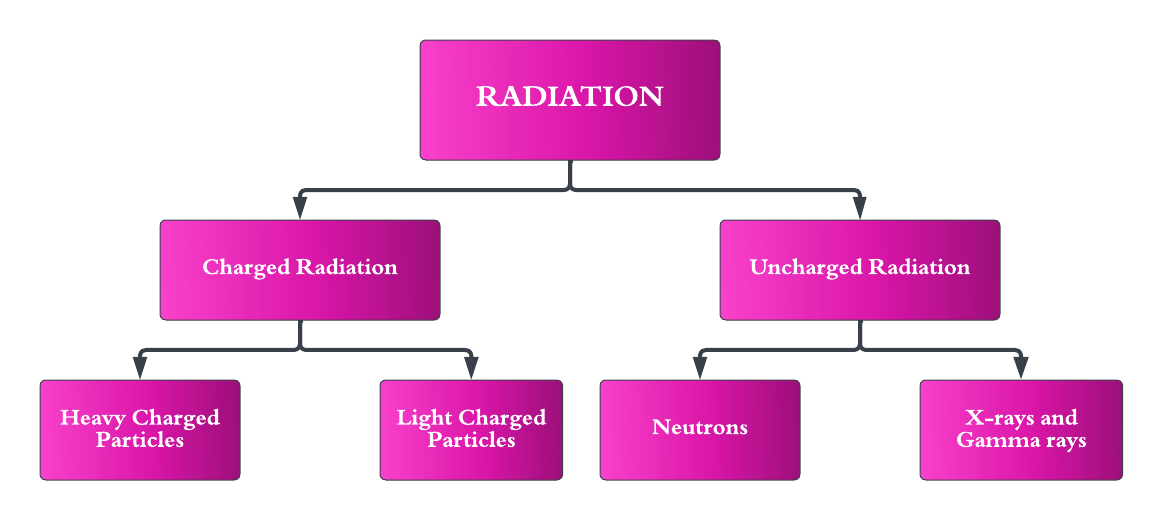
\includegraphics[width=0.8\linewidth]{RadiationClassification.png}
        \captionof{figure}{Classification of radiation}
        \label{fig:RadiationClassification}
    \end{Figure}

    \begin{itemize}
        \item \textbf{Uncharged Radiation} 

        \begin{enumerate}

            \item[A.)] \textbf{X-Ray and Gamma Rays}: Gamma Rays and X-rays interact with matter through 3 main processes :-

            \begin{enumerate}
                \item \textbf{Photoelectric Effect: } In this process, a photon undergoes an interaction with an absorber atom 
                in which the photon completely disappears. In its place, an energetic \textit{photo-electron} is ejected 
                by the atom from one of its bound shells. The energy of the photo-electron is given by:

                $$E_{e^-}=h \nu - E_b $$

                where E\textsubscript{b} is the binding energy of photo-electron in its original shell.

                \item \textbf{Compton Scattering: } In this process, the incoming \textgamma-ray photon strikes an electron 
                in the absorber medium and the \textgamma-ray is deflected through an angle $\theta$ with respect to its original 
                position. The photon transfers a portion of its kinetic energy to the electron, which is known as recoil electron. 
                The amount of energy transferred depends on the angle of scattering \straighttheta. The energy of the 
                scattered photon is given by:

                $$ h\nu^{'}=\frac{h\nu}{1+\frac{h\nu}{m_{0}c^{2}}(1-\cos{\theta})}$$

                where m\textsubscript{0}c\textsuperscript{2}  is the rest mass energy of electron.

                \item \textbf{Pair Production: } If the \textgamma-ray energy exceeds twice the rest-mass energy of electron 
                (1.02 MeV), the process of pair production is energetically possible. In this interaction, the \textgamma-ray 
                photon disappears and is	replaced by an electron-positron pair.
            \end{enumerate}

            \item[B.)] \textbf{Neutrons}: Neutrons are generally difficult to detect as their interaction with matter 
            is very less and can travel large distances without causing any interactions and hence can be detected only 
            through indirect methods depending on its speed. \textbf{\textit{Slow Neutrons }} do not directly interact with 
            detector atoms, however they have a high probability of causing neutron induced nuclear reactions which in turn 
            produce secondary particles/radiation which can be detected. While \textbf{\textit{Fast Neutrons} } with high 
            Kinetic Energies are mainly detected through scattering. For example, for reactions with moderators like hydrogen, 
            the recoil neutrons become secondary radiation. If Kinetic Energy of neutrons is sufficiently high, 
            inelastic collisions occur with detector atoms causing nucleus to excite to higher states, the excited nucleus 
            quickly de-excite to release radiation, which can then be detected. 
        \end{enumerate}

        \item \textbf{Charged Radiation} Charged particles interact with matter through \textit{Coulomb Forces} 
        between the radiation and the detector. These particles interact simultaneously with many electrons and in one 
        such encounter, the electron receives sufficient impulse from Coulomb force of the passing particle to excite 
        the electron to higher state (\textit{excitation}) or completely remove the electron from the atom 	
        (\textit{ionization}). The average energy loss is given by the \textbf{Bethe-Bloch}\cite{t1} formula:

        $$\frac{dE}{dx}=-K\frac{Z}{A}\frac{\rho}{\beta^2}\{ln\frac{2mc^2\beta^2E_M}{I^2(1-\beta^2)}\}$$

        where $\beta$ is the velocity (in units of c) of particle, 
        $K=\frac{2\pi Nz^2e^4}{mc^2}$ and $E_M=\frac{2mc^2\beta^2}{1-\beta^2}$ is the maximum energy transfer allowed.
        
    \end{itemize}
    
    \subsubsection*{\large Sources of Radiation}
        Sources of radiation can be categorized into two main groups \cite{u5}: natural sources and artificial (or man-made) sources. 
        The average annual radiation dose is shown in figure \ref{fig:SourcesOfRadiation}

        \begin{Figure}
            \centering
            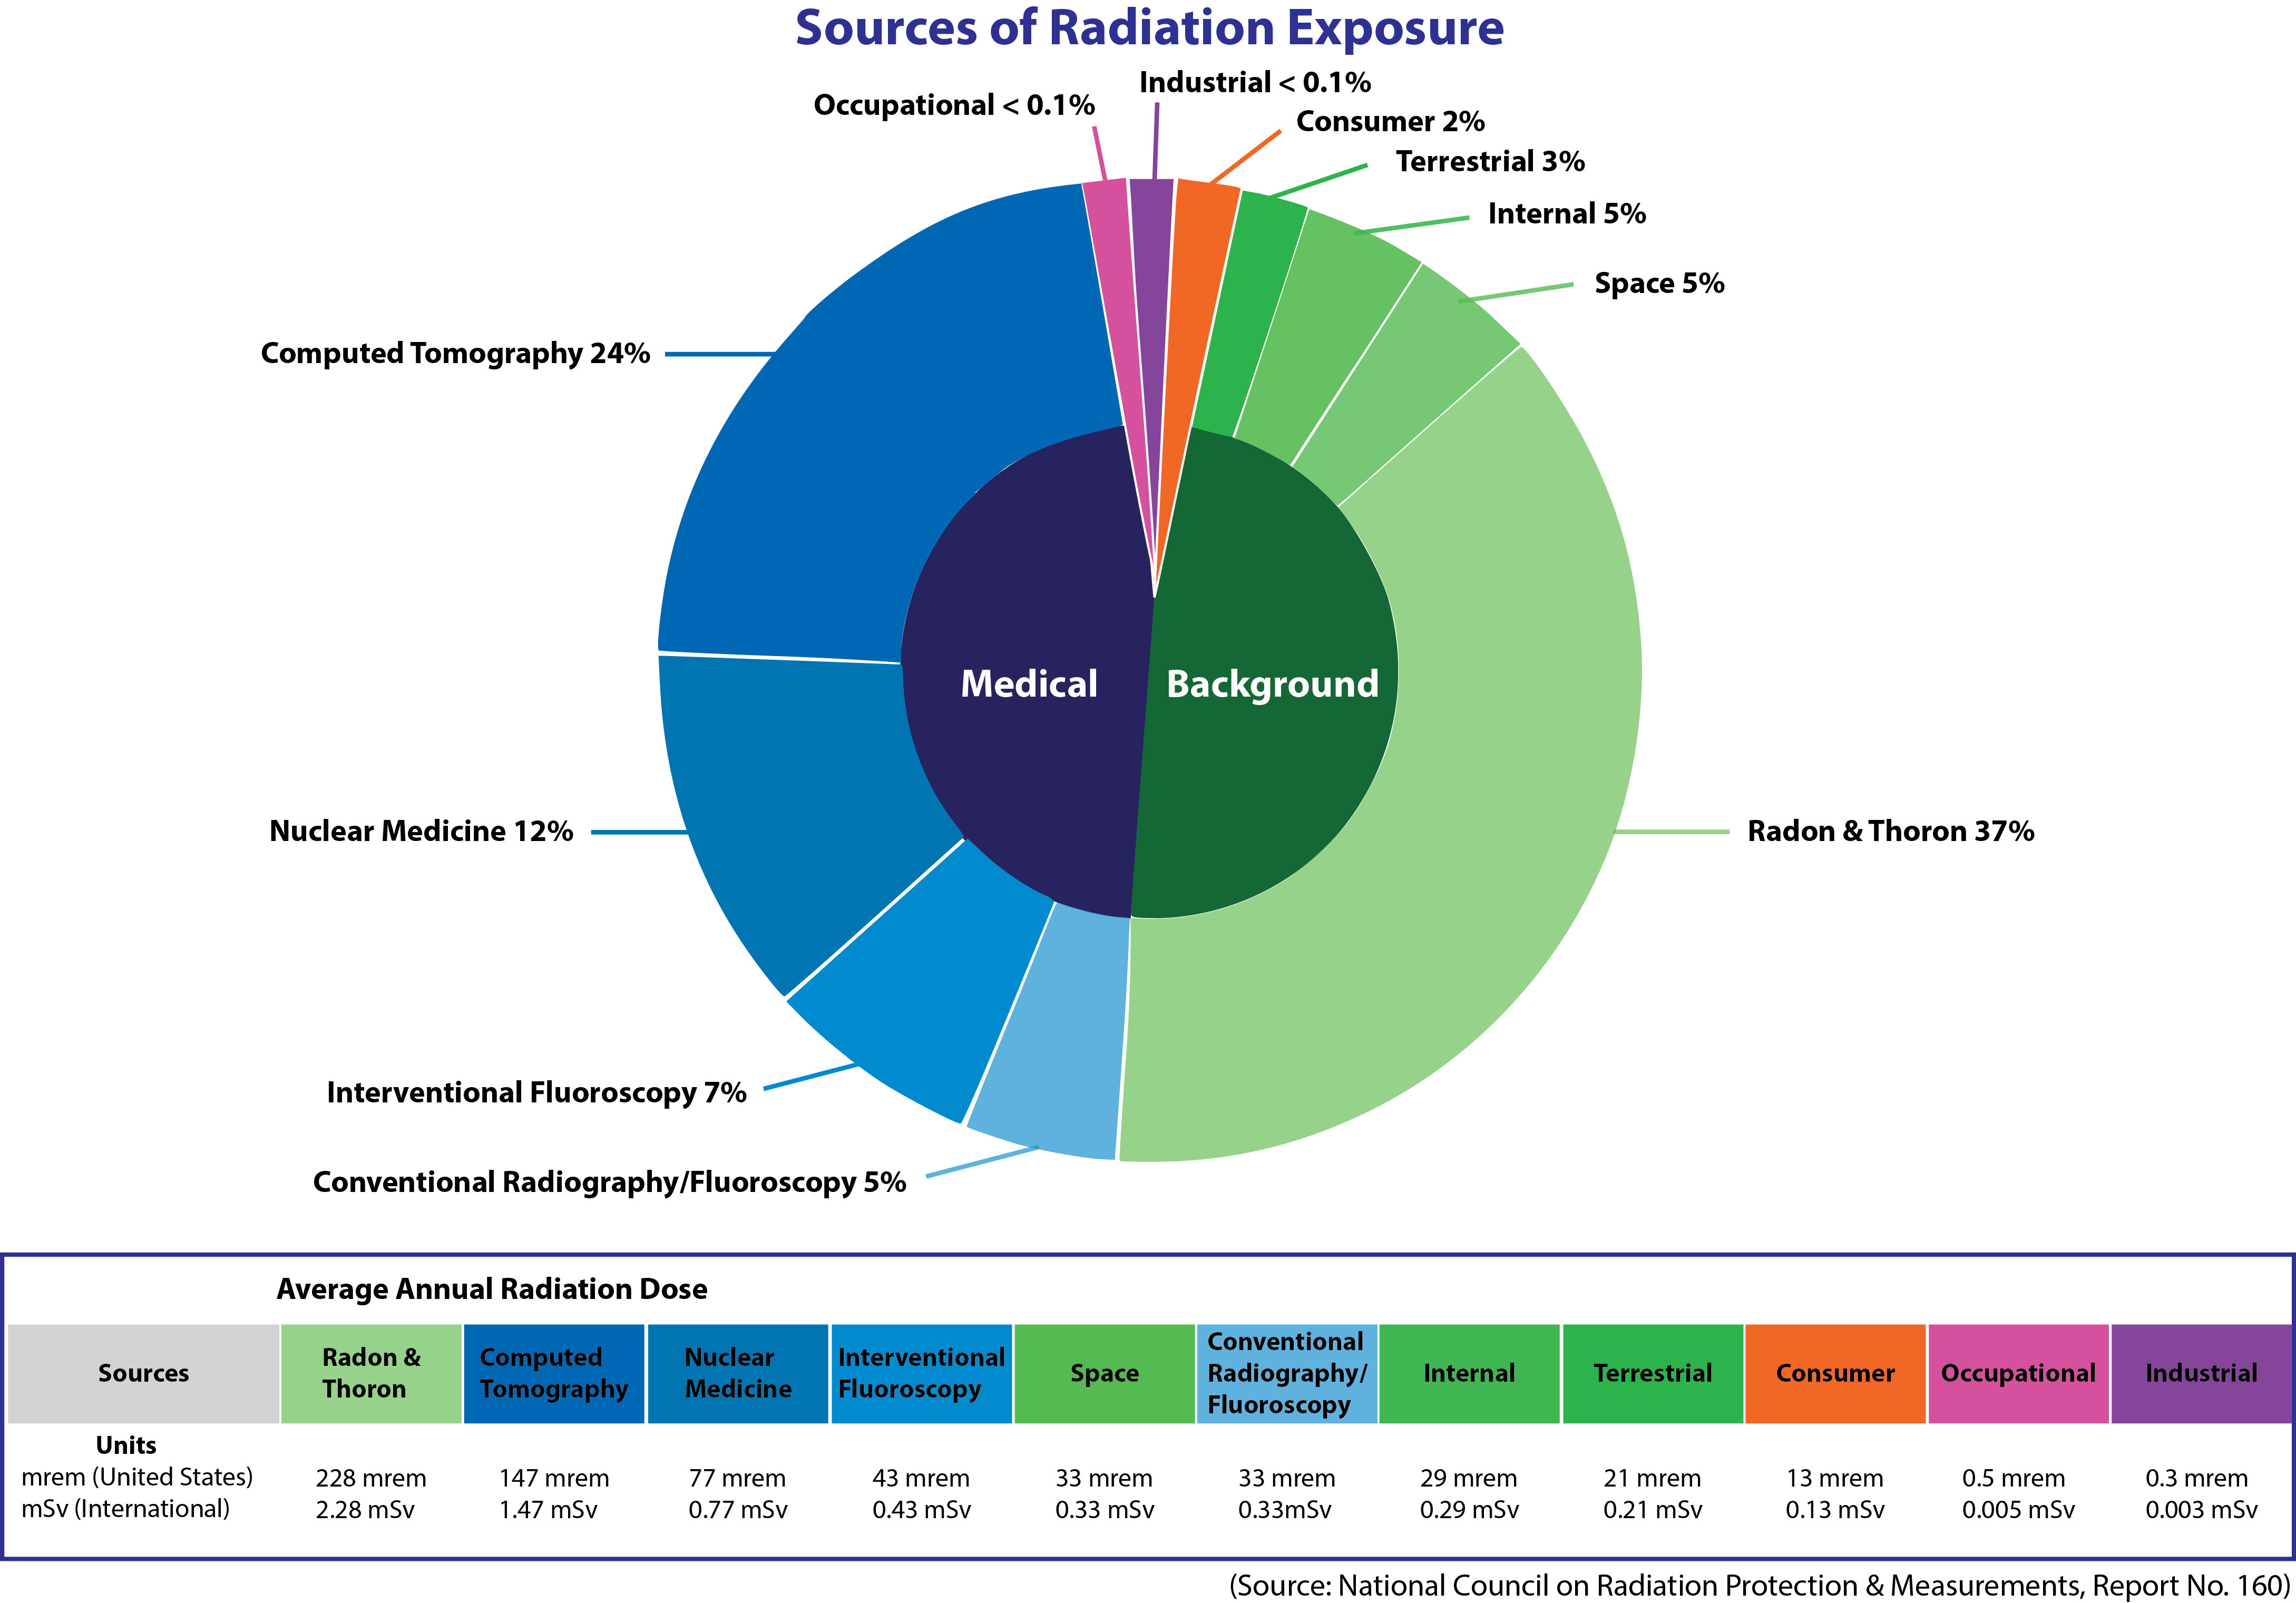
\includegraphics[width=0.8\linewidth]{SourcesOfRadiation.png}
            \captionof{figure}{Average Annual Radiation Dose\cite{a5}}
            \label{fig:SourcesOfRadiation}
        \end{Figure}

        \begin{enumerate}
            \item[A.)] \textbf{Natural Sources of Radiation:}
            \begin{itemize}
                \item \textbf{Cosmic Radiation:} High-energy particles, such as protons and atomic nuclei, that originate from outer space 
                and reach the Earth's atmosphere.

                \item \textbf{Terrestrial Radiation:} Naturally occurring radioactive elements present in the Earth's crust, such as uranium, 
                thorium, and radon gas.

                \item \textbf{Radon Gas:} A radioactive gas that is released from the decay of uranium and thorium in rocks, soil, 
                and water. It can accumulate in buildings, particularly in basements and poorly ventilated areas.

                \item \textbf{Radioactive Isotopes in the Environment:} Small amounts of radioactive isotopes, 
                such as potassium-40 and carbon-14, are naturally present in the environment and contribute to background radiation.

            \end{itemize} 

            \item[B.)] \textbf{Artificial (Man-Made) Sources of Radiation:}
            \begin{itemize}
                \item \textbf{Medical and Dental Procedures:} Diagnostic imaging techniques 
                like X-rays, computed tomography (CT) scans, and nuclear medicine procedures involve the use of ionizing radiation.

                \item \textbf{Radiation Therapy:}High-energy radiation, such as X-rays or gamma rays, used to treat cancer and other medical conditions.

                \item \textbf{Nuclear Power Plants:} Nuclear fission in reactors generates heat and electricity but also produces low-level radiation 
                during normal operation and potential radioactive releases during accidents.

                \item \textbf{Industrial Applications:} Industrial radiography, gauging, and research activities that involve the use of radiation 
                for inspection, measurement, and scientific experiments.
            \end{itemize}
        \end{enumerate}

        A chart depicting the levels of ionizing radiation is given below figure \ref{fig:LevelOfRadiation}
        \begin{Figure}
            \centering
            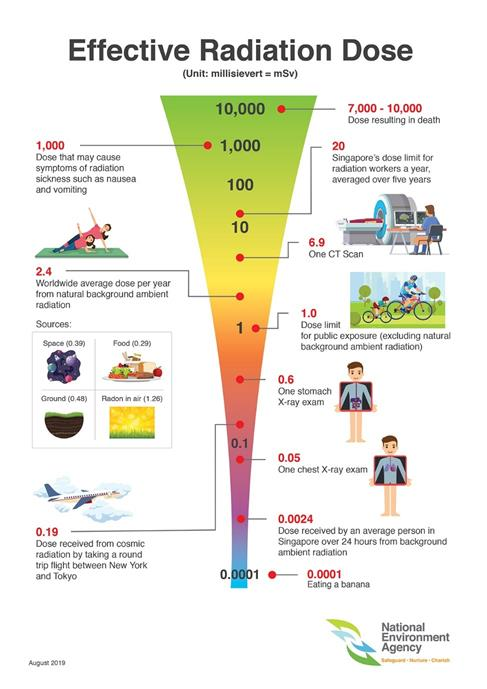
\includegraphics[width=0.5\linewidth]{LevelOfRadiation.jpg}
            \captionof{figure}{Effective Radiation Dose \cite{u2}}
            \label{fig:LevelOfRadiation}
        \end{Figure}


    \subsubsection*{\large Effects of Radiation}

        The effects of radiation on living organisms can be divided into two main categories: deterministic effects and 
        stochastic effects. These effects depend on various factors, including the type of radiation, the dose received, 
        and the duration of exposure. Here is an overview of the different effects of radiation:

        \begin{Figure}
            \centering
            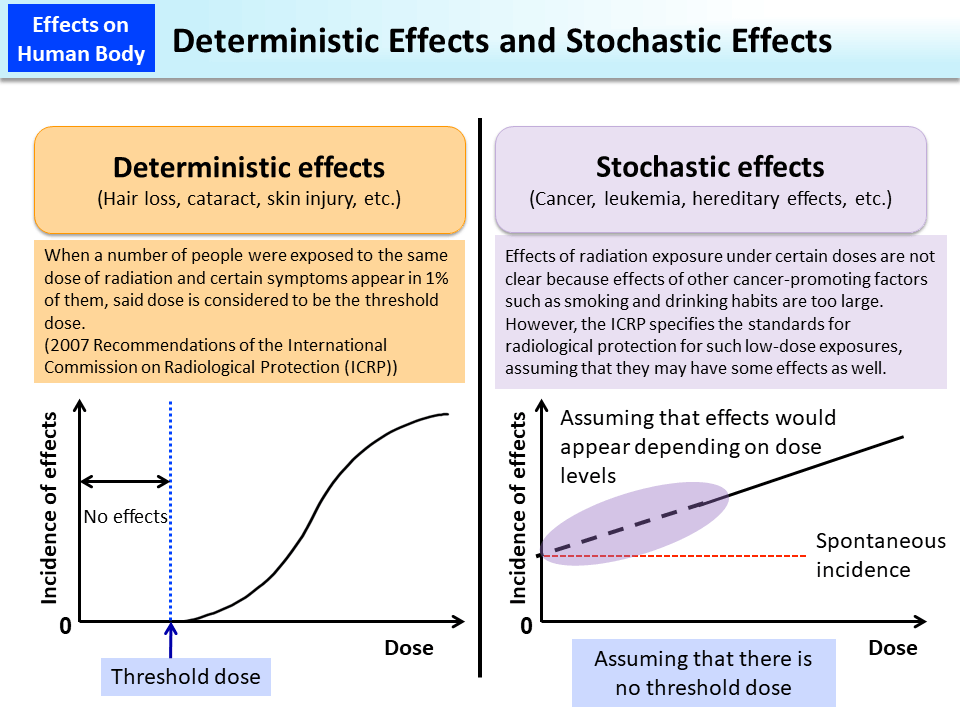
\includegraphics[width=0.8\linewidth]{EffectsOfRadiation.png}
            \captionof{figure}{Determinsitic and Stochaistic Effects of Radiation \cite{u3}}
            \label{fig:EffectsOfRadiation}
        \end{Figure}

        \begin{enumerate}
            \item[A.)] \textbf{Deterministic Effects:} Deterministic effects, also known as non-stochastic effects, occur when an 
            individual is exposed to high levels of radiation. These effects have a clear threshold dose below which no adverse effects are observed. 
            As the dose increases above the threshold, the severity of the effects increases. Key deterministic effects include:

            \begin{itemize}
                \item \textbf{Radiation Sickness:} At high doses, radiation can cause radiation sickness, also known as acute radiation syndrome. 
                Symptoms may include nausea, vomiting, fatigue, diarrhea, loss of appetite, and decreased blood cell counts. 
                The severity and onset of symptoms depend on the radiation dose received.

                \item \textbf{Skin Burns:} High doses of radiation can cause severe burns on the skin, similar to thermal burns. 
                These burns can be painful and may require medical attention.

                \item \textbf{Organ Damage:} Radiation exposure can result in damage to specific organs, such as the gastrointestinal system, 
                cardiovascular system, and reproductive organs. The severity of organ damage depends on the dose received and the sensitivity of 
                the organ to radiation.

            \end{itemize} 

            \item[B.)] \textbf{Stochastic Effects:}
            Stochastic effects, also called probabilistic effects, are random in nature and occur without a clear dose threshold. 
            They are associated with long-term exposure to low or moderate doses of radiation. The probability of these effects occurring 
            increases with higher radiation doses, but their occurrence is not guaranteed. Key stochastic effects include:

            \begin{itemize}
                \item \textbf{Increased Risk of Cancer:} Prolonged exposure to radiation, even at low doses, can increase the risk of 
                developing cancer. Ionizing radiation has the potential to damage DNA, leading to genetic mutations that can 
                initiate cancerous growth. The types of cancer that may develop depend on the irradiated organs and tissues.

                \item \textbf{Hereditary Effects:} Radiation exposure can also affect future generations. High doses of radiation to 
                reproductive cells (sperm or eggs) can increase the risk of genetic mutations and hereditary disorders in offspring.

            \end{itemize}
        \end{enumerate}

        It is important to note that the likelihood and severity of both deterministic and stochastic effects depend on factors such as the 
        type of radiation (e.g., gamma rays, alpha particles), the duration of exposure, and the sensitivity of the exposed individual or organism.
        To protect individuals and mitigate the effects of radiation, radiation protection guidelines and regulations are implemented 
        in various fields, including medicine, industry, and nuclear power. These measures aim to minimize radiation exposure, optimize radiation 
        practices, and ensure the safety of workers and the general public.

    \subsubsection*{\large Applications Of Radiation}
        Radiation has numerous applications across various fields, including medicine, industry, agriculture, research, and energy production. 
        Here are some notable applications of radiation:
        
        \begin{itemize}
            \item \textbf{Medical Imaging:} Radiation is widely used in medical imaging techniques to diagnose and monitor diseases. X-rays and 
            computed tomography (CT) scans utilize ionizing radiation to create detailed images of the body's internal structures, aiding in the 
            detection of fractures, tumors, and other abnormalities.

            \item \textbf{Radiation Therapy:} Radiation therapy, also known as radiotherapy, is a common treatment modality for cancer. 
            High-energy radiation, such as X-rays or gamma rays, is precisely targeted to destroy cancer cells and shrink tumors. Techniques like 
            external beam radiation therapy and brachytherapy are used to deliver radiation to specific areas of the body.

            \item \textbf{Nuclear Medicine:} In nuclear medicine, small amounts of radioactive substances called radiopharmaceuticals are 
            administered to patients for diagnostic and therapeutic purposes. These substances emit gamma rays that can be detected by imaging 
            devices to create functional images of organs and tissues, aiding in the diagnosis and treatment of various conditions.

            \item \textbf{Industrial Applications:} Radiation is utilized in various industrial applications, including non-destructive testing (NDT) 
            and quality control. Radiography techniques, such as X-ray and gamma-ray imaging, are employed to inspect welds, detect flaws in 
            structures, and assess the integrity of materials without damaging them. Radiation is also used for sterilization of medical equipment, 
            food preservation, and insect control in agriculture.

            \item \textbf{Research and Scientific Studies:} Radiation plays a crucial role in scientific research, enabling scientists to study 
            the properties and behavior of materials, molecules, and subatomic particles. Techniques such as X-ray crystallography, 
            neutron scattering, and positron emission tomography (PET) are employed to investigate the structure, composition, and dynamics of 
            various substances.

            \item \textbf{Energy Production:} Nuclear power plants generate electricity by harnessing the energy released from nuclear reactions. 
            Controlled fission of radioactive isotopes, such as uranium-235, produces heat, which is then converted into electrical energy. 
            Nuclear energy provides a reliable and low-carbon source of power, contributing to the global energy mix.

            \item \textbf{Radiation Therapy for Food Preservation:} Ionizing radiation is used to preserve food by inhibiting the growth of bacteria, 
            molds, and insects. This technique, known as food irradiation, can extend the shelf life of perishable foods, improve food safety, and 
            prevent the spread of foodborne illnesses.

        \end{itemize}

        It is worth noting that the application of radiation is carefully regulated to ensure safety and minimize potential risks. 
        Strict guidelines, protocols, and safety measures are in place to protect individuals, the environment, and public health in all areas 
        where radiation is used.
    
    \subsubsection*{\large Radiation Protection and Safety}
        Radiation protection and safety encompass a range of measures and practices aimed at minimizing radiation exposure and ensuring the 
        safety of individuals, the public, and the environment \cite{b3}. The principles of radiation protection are based on the \textbf{ALARA} principle, 
        which stands for \textit{"As Low As Reasonably Achievable."} as sfown in figure \ref{fig:RadiationSafety}\

        \begin{Figure}
            \centering
            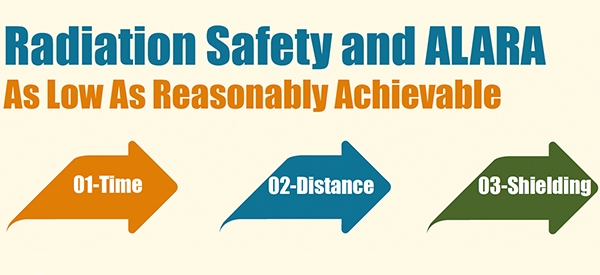
\includegraphics[width=0.8\linewidth]{RadiationSafety.jpg}
            \captionof{figure}{Principle of ALARA \cite{u4}}
            \label{fig:RadiationSafety}
        \end{Figure}

        
        
        Here are some key aspects of radiation protection and safety:
        \begin{itemize}
            \item \textbf{Dose Limits:} Regulatory authorities and international organizations establish dose limits that specify the maximum 
            allowable radiation doses for individuals in different contexts. These limits vary depending on factors such as occupation, 
            public exposure, and medical procedures. Compliance with dose limits is essential to prevent excessive radiation exposure.

            \item \textbf{Risk Assessment and Management:} Radiation risks are assessed and managed by conducting thorough risk assessments. 
            This involves evaluating the potential hazards associated with radiation sources, estimating the likelihood and magnitude of 
            exposures, and implementing appropriate control measures to mitigate risks.

            \item \textbf{Shielding and Containment:} Shielding materials, such as lead, concrete, and steel, are used to attenuate radiation 
            and protect individuals from exposure. Proper shielding design and construction are crucial in areas where radiation sources are 
            used, such as medical facilities and nuclear power plants. Additionally, containment measures ensure that radioactive materials are 
            safely stored and handled to prevent their release into the environment.

            \item \textbf{Personal Protective Equipment (PPE):} Personal protective equipment, such as lead aprons, gloves, and goggles, is 
            utilized to protect individuals who work with or around radiation sources. PPE helps to reduce radiation exposure to specific body 
            parts and ensures that workers adhere to safety protocols.

            \item \textbf{Training and Education:} Comprehensive training and education programs are essential for individuals who work with 
            radiation sources. This includes radiation safety training, radiation protection protocols, proper handling and storage of 
            radioactive materials, and emergency response procedures. Continuous education and awareness campaigns help maintain a strong 
            safety culture.

            \item \textbf{Monitoring and Dosimetry:} Regular monitoring of radiation levels and individual doses is conducted to ensure 
            compliance with safety standards and detect any potential overexposures. Dosimeters, such as \textbf{Thermoluminescent dosimeters (TLDs)} 
            and electronic personal dosimeters (EPDs), are used to measure and record radiation doses received by individuals.

            \item \textbf{Regulatory Compliance and Inspections:} Regulatory bodies oversee and enforce radiation safety regulations. 
            They conduct inspections, audits, and assessments to ensure that radiation practices comply with safety guidelines. 
            Non-compliance can result in penalties, fines, or the suspension of operations.

            \item \textbf{Emergency Preparedness and Response:} Preparedness for radiation emergencies, such as accidents or incidents involving 
            radiation sources, is crucial. Emergency response plans, evacuation procedures, and communication protocols are established to 
            protect the public and mitigate the consequences of such incidents.

        \end{itemize}
        It is important to note that radiation protection and safety require a multidisciplinary approach involving collaboration among 
        regulatory bodies, radiation safety officers, medical professionals, researchers, and workers handling radiation sources. 
        Continuous improvement, adherence to best practices, and staying up-to-date with advancements in radiation protection are vital to 
        ensuring the safe and responsible use of radiation.

\end{document}